\documentclass{sigchi}

% Use this command to override the default ACM copyright statement (e.g. for preprints). 
% Consult the conference website for the camera-ready copyright statement.


%% EXAMPLE BEGIN -- HOW TO OVERRIDE THE DEFAULT COPYRIGHT STRIP -- (July 22, 2013 - Paul Baumann)
% \toappear{Permission to make digital or hard copies of all or part of this work for personal or classroom use is granted without fee provided that copies are not made or distributed for profit or commercial advantage and that copies bear this notice and the full citation on the first page. Copyrights for components of this work owned by others than ACM must be honored. Abstracting with credit is permitted. To copy otherwise, or republish, to post on servers or to redistribute to lists, requires prior specific permission and/or a fee. Request permissions from permissions@acm.org. \\
% {\emph{CHI'14}}, April 26--May 1, 2014, Toronto, Canada. \\
% Copyright \copyright~2014 ACM ISBN/14/04...\$15.00. \\
% DOI string from ACM form confirmation}
%% EXAMPLE END -- HOW TO OVERRIDE THE DEFAULT COPYRIGHT STRIP -- (July 22, 2013 - Paul Baumann)


% Arabic page numbers for submission. 
% Remove this line to eliminate page numbers for the camera ready copy
% \pagenumbering{arabic}


% Load basic packages
\usepackage{balance}  % to better equalize the last page
\usepackage{graphics} % for EPS, load graphicx instead
\usepackage{times}    % comment if you want LaTeX's default font
\usepackage{url}      % llt: nicely formatted URLs
\usepackage{epstopdf}
\usepackage{listings}

\makeatletter
\newif\if@restonecol
\makeatother
\let\algorithm\relax
\let\endalgorithm\relax
\usepackage[ruled,vlined]{algorithm2e}



% llt: Define a global style for URLs, rather that the default one
\makeatletter
\def\url@leostyle{%
  \@ifundefined{selectfont}{\def\UrlFont{\sf}}{\def\UrlFont{\small\bf\ttfamily}}}
\makeatother
\urlstyle{leo}


% To make various LaTeX processors do the right thing with page size.
\def\pprw{8.5in}
\def\pprh{11in}
\special{papersize=\pprw,\pprh}
\setlength{\paperwidth}{\pprw}
\setlength{\paperheight}{\pprh}
\setlength{\pdfpagewidth}{\pprw}
\setlength{\pdfpageheight}{\pprh}

% Make sure hyperref comes last of your loaded packages, 
% to give it a fighting chance of not being over-written, 
% since its job is to redefine many LaTeX commands.
\usepackage[pdftex]{hyperref}
\hypersetup{
pdftitle={SIGCHI Conference Proceedings Format},
pdfauthor={LaTeX},
pdfkeywords={SIGCHI, proceedings, archival format},
bookmarksnumbered,
pdfstartview={FitH},
colorlinks,
citecolor=black,
filecolor=black,
linkcolor=black,
urlcolor=black,
breaklinks=true,
}

% create a shortcut to typeset table headings
\newcommand\tabhead[1]{\small\textbf{#1}}


% End of preamble. Here it comes the document.
\begin{document}

\title{What and to what extent you have read: understanding your daily online learning process}

\numberofauthors{3}
\author{
  \alignauthor Lei Zhang\\
    \affaddr{Georgia State University}\\
    \affaddr{Atlanta,Georgia,U.S.A}\\
    \email{lzhang14@student.gsu.edu}
  \alignauthor Ying Zhu\\
    \affaddr{Georgia State University}\\
    \affaddr{Atlanta,Georgia,U.S.A}\\
    \email{yzhu@cs.gsu.edu}
}

\maketitle

\begin{abstract}

In this paper, we present our research on detecting habitual reading region 
on the screen when a user is doing his daily online reading. Instead of traditional eye-tracking based solution,
we developed an unintrusive user attention tracking(UUAT) solution. In UUAT, we developed a ReadingClue 
technology,  which helps to pinpoint user reading attention when necessary. At the same time, user reading behavioral data(mouse click and mouse scroll) is
collected in background. With these behavioral data, UUAT calculates a user's preferred reading region. Our experiment
indicates that the accuracy of UUAT attention tracking is as high as 93.2\%.





\end{abstract}

\keywords{
	Attention Tracking; Reading; Mouse movements; Scrolling;
}

\category{H.5.m.}{Information Interfaces and Presentation (e.g. HCI)}
{Miscellaneous}

\section{Introduction}

Personal Data Mining\cite{ozzie2011personal}(PDM) has been proposed as a complement to commercial/business data mining. While commercial data mining\cite{berry1997data} often aims to discover new knowledge to improve business opportunity or maketing strategies,  PDM is proposed for a user’s individual good. In PDM, user behavioral data is collected by a neutral utility, and it is under the user's full control. The user can choose third-party tools(local) or service(cloud) to analyze his personal data, aiming to improve individual productivity or life quality. Besides being mined alone, individual's behaviroal data can be analyzed with data from other users to find correlations among the data or similar users(e.g. User with similar interests).

 
As the first step of PDM, detailed and objective raw personal data should be collected. Self-Tracking\cite{swan2009emerging,wolf2010data} is getting increasingly popular to log personal data, so that future analysis can be conducted for a user’s good in health. Self-Tracking has been mainly involved in personal physical data, such as, weight, heartbeat, diet and sports. Moreover, the way of logging data has been mainly referred to manual logging, e.g. a user input his weight before going to bed everyday. However we argue that the reign of personal data is broder than physical data and the ways to collect personal data can be extended to an automatic and unaware way. 


In this research, we consider a user’s daily reading as a source of personal data. An immediate reason is that understanding a user's daily reading helps to build a user’s personal knowledge database, let alone "For many self-trackers, the goal is unknown"\cite{wolf2010data}. To be specific, we do not consider reading of an artilce as a simple-and-plain data item (e.g one record to log the tittle, url, timestamp,etc ). Instead, we consider it to be richer informational process , where potentially we can discover much more knowledge. For example, during the reading process, if a user spent more unit reading time on a specific paragraph  than average(no distraction), this indicate that the user might have pondered on the information in that paragraph or have reading struggles on paragraph one. In either case, it might indicate that the user has encountered new knowledge and he takes time to digest this new information. Another example is that, if a user skims very fast over a paragraph, it is very likely that he is not interested in the information provided by that paragraph.  From this point of view, it might be a mileage for personal knowledge acquisition, e.g., today is the day I first come to know the concept of “shale gas”(I read and pondered on the paragraph), although I have read the same phrase years ago(I skimmed over that paragraph very fast). To enable this type of knowledge discovery and to record this type of personal data, it is unlikely to adopt the existing user-aware solutions(e.g. eye-trackiing or self-tracking), a smart and intelligent collection method is required to obtain personal reading data. 


In this research, we focus on how to collect detailed  and objective reading behavioral data, so that PDM can be conducted on an accurate and correct basis. To be specific, we focus on a user’s daily online reading activity. Our goal is as follows: in a finer granularity,   
we accurately identify what texts a users read and to what extent he has spent on specific parts of an article. To realize this goal, we developed a browser-based attention tracking system, namely UUAT, to collect daily reading behavioral data. UUAT collects a user's
interaction data during his reading, then it computes user's behavioral reading region and finally provides reading details of that reading event. In this way, we enable a more extensive PDM applications which we present in future work section. Our contributions are as follows: 1. To the best of our knowledge, we first compute the user preferred reading region in an unaware but accurate way. 2. We monitor a user's reading and produce detail, meaningful, and objective data, which can be used as input for deep PDM.


\section{Related Work}

The idea of quantified self-tracking is well known proposed in \cite{wolf2010data}. In \cite{wolf2010data}, the author advocates collecting individual quantified data. He presents cases where individual data collection helped to solve person-specific problems. For example, Barbier used her daily logged personal data to find a way to cure her insomnia\cite{wolf2010data},  Seth Roberts, a Caltech professor, analyzed his personal data and find an optimum diet(flaxseed oil) to improve his math performance\cite{wolf2010data}. In this work, the author advocates a diversified personal data collection, as long as the data is quantified, albeit you might not know the goal of your data collection immediately. The current state-of-art personal data mainly includes personal physical data, such as weight, glucose, heartbeat, sports, food/medication consumption. So the existing pervasive methods of personal data collection are mainly by a user himself, such as the methods adopted by PatientsLikeMe\cite{plm}, a user/patient input his biological data into his computer(usually a spreadsheet) and save it for future use.  Our research adopts an user-unaware, automatic method to collect a user's personal data. 



Our first research goal is the computation of a user's preferred reading region, the literature in this research field can be mainly divided into two catagories. Eye-Tracking based research and mouse/keyboard 
tracking based research.


\cite{nielsen2010eyetracking} is a typical eye-tracking based research. The author used eye-tracking to find out that a user's attention region and cursor are closely related, 
both of them can be modeled as a normal distribution.  We argue that eye-tracking based methods are also tagged as intrusive and expensive. On the one hand,
the behavior of subjects wearing a headset might be biased from his natural behavior. On the other hand,  it is impractical to popularize an eye-tracking based application to a large scale,
especially when a pervasive self-tracking is referred. 

Compared to eye-tracking method, our research is closer to the work of \cite{navalpakkam2012mouse,huang2011no,lagun2011viewser,atterer2007tracking,hornbaek2003reading,atterer2008heatmap}
The work in \cite{atterer2008heatmap} developed a vertical heatmap bar for long webpage viewers, indicating the dwell time of each specific part of web page.
 This paper collects similar data as us (user scroll), but aims at a different goal: to navigate user when he want to read backwards. 
The work in \cite{hornbaek2003reading} developed compared the different reading assistance technologies, and find out the improvement on reading from each technology.
Our work is different from \cite{atterer2008heatmap,hornbaek2003reading} that we do not intend to assist a user's reading process(navigation or improve reading efficiency),
 we aims to develop an "observer", which can get objective and accurate user reading behavioral data. 

The authors of \cite{navalpakkam2012mouse} collected user mouse data, at the same time they collected user’s eye gaze data, they proved that the user mouse data can indicate user behavior, e.g. which part of the screen is more attractive, the user distraction behavior can be detected and the user experience can be predicted by mouse analysis in an accuracy of 80%. The result of this research  highly depends on the eye-gaze data and again we argue that the user behavior might be changed once a subject is put into a headset device and knowing he might be taped in a video. The research of \cite{atterer2007tracking} are conducted in a goal of software usability test. They collect user data in an unaware way, which is more objective. The collected data is very detail focused, which might be used to construct a “playback” for a tester’s tryout. The downside of this research is that it needs to log every interaction between a user and a web component(not a web page, but each HTML components in that webpage),  e.g. how long does it take the subject to first click on a specific radio button on a page. This makes it a difficult knowledge in the context of web2.0. So a further research\cite{atterer2006knowing} is conducted on how to log user interaction with Ajax-based web components. Since the research goal is to evaluate a software usability, the work in \cite{atterer2007tracking,atterer2006knowing} collects data in a raw and  particular way. Furthermore, extra server-side support is needed to conduct the data collection, making it less scalable. The research of \cite{huang2011no} are conducted for evaluation of search engine result pages. Both of them collect data for the goal to discover which search engine result item is more attractive to a user. In \cite{huang2011no}, the author proposed a “viewport” technology, which blurs all the other result items except one item, so that the user can put his attention on result item. In this way, the user is forced to locate his reading region to where the unblurred item is.  In \cite{lagun2011viewser}, the author also tries to make use of mouse data, but they are more interested in the mouse trajectory instead of the mouse click, since the mouse is more often to move in the screen than a mouse is clicked, but the mouse move does not always trigger an event that can be logged. With the comparison of eye-gaze data, they disclose that the mouse trajectory can be used to infer a user’s interest on the search engine result items.


By literature review we distinguish our research from existing works as follows: the data collection in our research is designed to be more scalable, so our data collection method can be tagged as "unintrusive", unlike the eye-gaze technology adopted in \cite{navalpakkam2012mouse,lagun2011viewser}. Meanwhile our goal is personal data collection instead of usability test, we proposed a new CHI technology to accurately infer user’s preferred reading region on the screen, so that we can collect high quality data that can describe a user’s daily reading behavior objectively. 


The review for knowledge discovery 




\section{Where do you read?}
To understand  online reading in an user-unaware way, it is necessary to determine a user's Reading Region(RR). A Reading Region is defined as
the screen area where a user's reading attention effectively covers. Only those texts in the  RR are possibly read and learnt by a user. In this section we 
will first model RR and introduce our method to compute behavioral RR and realtime RR.

\subsection{Model of Reading Region}
Psycologically, felt involvement\cite{celsi1988role} influences attention and comprehension.  Felt involvement is low when a person starts reading any text. 
but it increases rapidly as reading continues until felt involvement reaches a peak value. After that, felt involvement decreases due to a decrease in the attentional
resources. The hypothesis in  \cite{celsi1988role} can also be proved by \cite{buscher2010eye}. 

The previous research on user attention tracking \cite{buscher2010eye} have disclosed some facts when a user is doing daily reading on 
long articles and documents. Vertically, in most of the time, the reading progresses towards the end of the screen  in a line-by-line manner. 
However, the reading does not start from the first line on the screen to the last line of the screen. Generally, a user has a preferred reading region on screen, which in this paper, 
we name it as behavioral RR(BRR), as indicated in figure \ref{fig:read_region}. A BRR can be identified by two parameters $\Delta$ and $w_0$. $\Delta$  indicates the 
offset from the head of the screen and $w_0$ indicates the vertical span of the whole region. If a user wants to read the contents outside the RR,
a scroll action is expected. In this research, we take aforementioned assumption and model the user attention region as displayed in figure \ref{fig:read_region}. 


\begin{figure}[!h] 
\centering
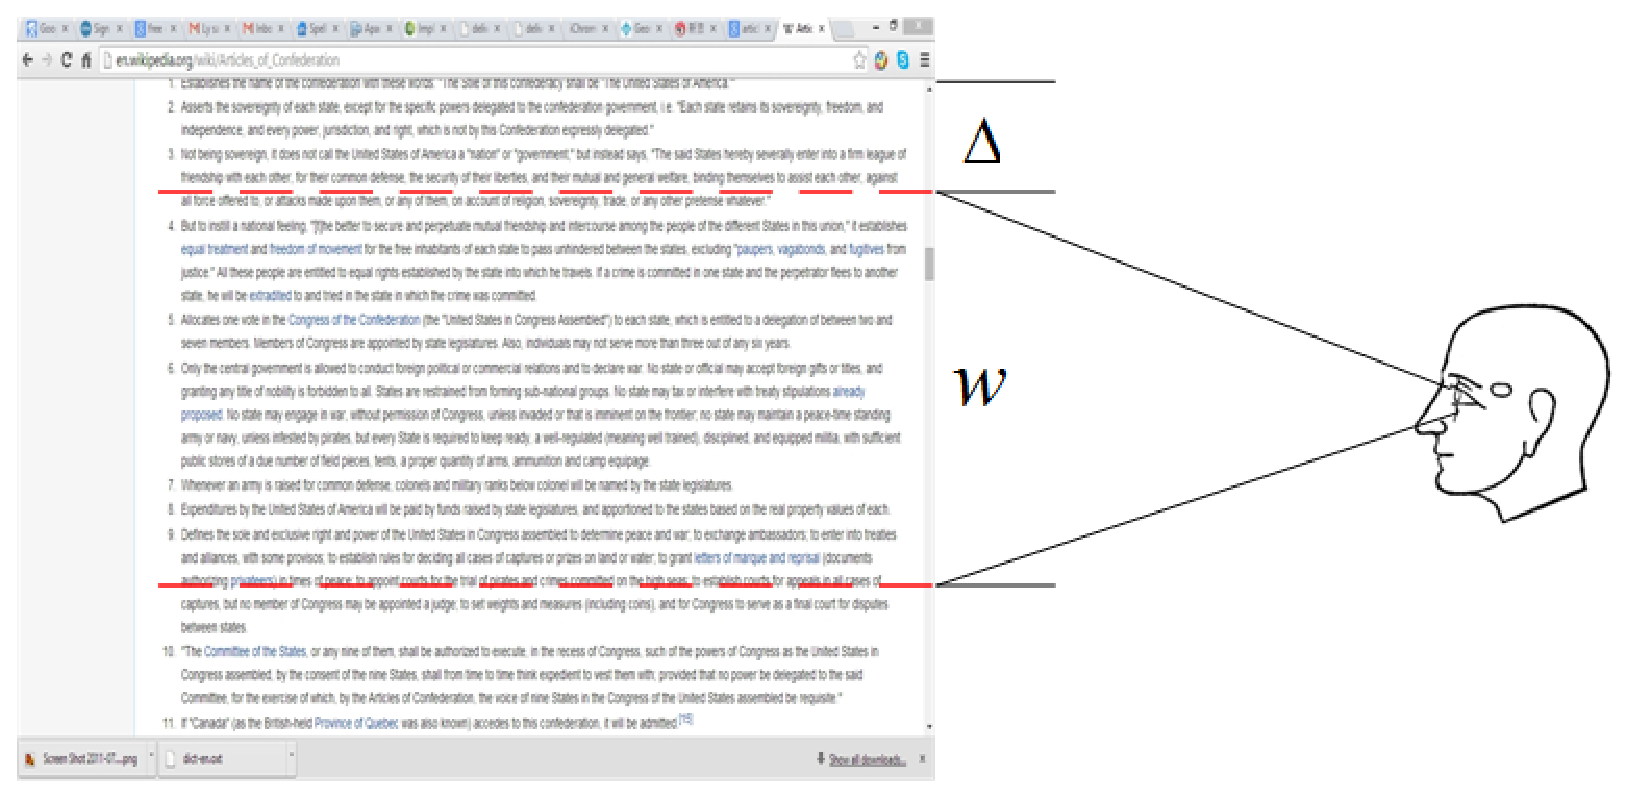
\includegraphics[width=1.0\columnwidth]{pictures/preferred_reigon}
\caption{The preferred reading region on the screen}
\label{fig:read_region}
\end{figure}

Taking this model into consideration, our next  research question is: 
What behavioral data should be collected and analyzed to compute RR?

Eye tracking data can be easily mentioned to answer the question, especially when a "visual" reading region is 
the goal. However, we argue that the eye tracking data has twofold major drawbacks: 1. The eye tracking collection 
requires extra hardware, which means the eye tracking  based solution  is not scalable and very costly. 2. What is even worse, 
eye tracking is "intrusive". A subject person is aware that he is wearing a headset device and he is under a camera coverage, 
his behavior is very likely to be different from how he behaves when he is doing reading alone. For these two reasons, we 
can not use eye tracking data. To meet the requirement of inattentive but objective, the only option left is the user interaction data 
collected when the reading is ongoing.  In the next subsection we will discuss how to collect and analyze user
 interaction data to get the user preferred region. 


\subsection{Calculating BRR by Interaction Data}

When a user is doing daily reading, since the keyboard input rarely happens 
during the reading process,  we are more interested in the mouse-generated data. 
There are two categories of mouse-generated data, click and scroll.  We consider the mouse-generated data to be 
informational  behavioral data. To be specific, an intentional  mouse click indicates 
the position of user's instantaneous reading attention, 
while a page scroll indicates how much contents has been moved out of reading region.

In this subsection, we answer the question of how to infer BRR by mouse-generated data. To be specific, 
according to figure \ref{fig:read_region},  RR can be identified by two parameters $\Delta$ and $w_0$. So
the computation of BRR can be transformed to how to compute  $\Delta$ and $w_0$.


Now we examine a typical online reading event, during which a user finishes reading of a whole article. We suppose 
the article is relatively long, which requires many scroll actions. 
The whole reading process can be illustrated by figure \ref{fig:scroll}

\begin{figure*}[t]
\centering
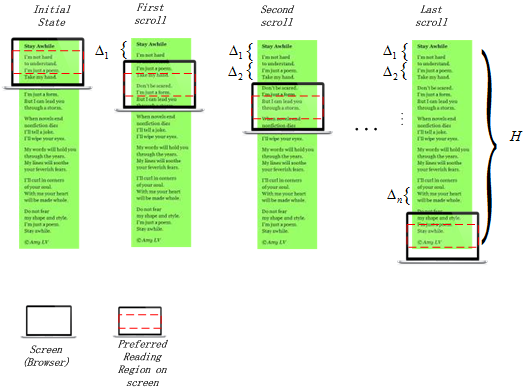
\includegraphics[width=1.5\columnwidth]{pictures/scroll}
\caption{Reading of a long article in a browser}
\label{fig:scroll}
\end{figure*}




In figure \ref{fig:scroll}, a user conducts a scroll action when he has finished reading contents of current reading region. 
At $i$th scroll action, a $w_i$ of page height will be moved out of region. So when the article reading is finished, 
we have equation (\ref{eq:1}). In equation (\ref{eq:1}) , $\Delta$ and $w_0$ are defined in figure 
\ref{fig:read_region}. Ideally, equation (\ref{eq:2}) should hold and the parameter $w_0$ can be 
calculated in equation (\ref{eq:3}). In practice, it is unlikely for equation (\ref{eq:2}) to strictly hold,
however, equation (\ref{eq:1}) can still be applied. 

\begin{equation} \label{eq:1}
	H = \sum\limits_{i = 1}^n {{w _i} + {\Delta } + w_0}  
\end{equation}

\begin{equation} \label{eq:2}
	{w _1} = {w_2} = ... = {w_n} = {w_0}
\end{equation}

\begin{equation} \label{eq:3}
	w_0 = \frac{{\sum\limits_{i = 1}^n {{w _i}} }}{n}
\end{equation}

With equation \ref{eq:3}, we can compute  $w_0$ parameter of a user's behavioral reading region(BRR). 
The computation of $\Delta$ can not be accomplished if only the scroll data is considered. Here we take
the mouse click data into consideration.Since we take the assumptions that the reading process progresses 
line by line and the mouse click is an indication of instantaneous user attention, we take the first click after each scroll as the clue to compute $\Delta$.


We note the click data $K$ as a sequence $K=(K_0,K_1,...,K_n)$, where 
there are $n$ scrolls and the component $K_i$ is the click sequence collected 
after $i_{th}$ scroll. Furthermore, $K_i= (K_i^0,K_i^1,....)$ and $K_i^j$ consists
of timestamp and coordinates, $< {t_{k_i^j}},{x_{k_i^j}},{y_{k_i^j}}>$. So we 
can compute $\Delta$ as following equation:

\begin{equation} \label{eq:31}
\Delta  = \frac{{\sum\limits_{i = 0}^n {{y_{k_i^0}}} }}{{n + 1}}
\end{equation} 

Once we compute $\Delta$ and $w_0$, we can have a good estimation of BRR. BRR can be considered as 
relatively stable. During the reading process in real time, BRR can be used to estimate the reading region if not 
enough information is provided. Due to the variation, equation (\ref{eq:2}) does not always hold, a realtime reading
region(RRR) should be computed at each scroll action, especially when the variation among scrolls are relatively large. 

\subsection{ Calculating RRR by Interaction Data }

Since equation (\ref{eq:2}) does not always hold, if the variance of $w_i$ is relatively large(actually it is),
we need to consider the question how to infer user reading  region on each single scroll. Figure \ref{fig:single_click}
displays the events happened during  reading between two scroll actions. Here solid dots are collected mouse click data with
the position on the corresponding place on the screen. Since we take the assumptions that the reading process progresses 
line by line and the mouse click is an indication of instantaneous user attention, we can calculate a minimum reading region after $i_{th}$ scroll action, 
$w_i^{\min }$, which can be identified by highest click and lowest click(as indicated in figure \ref{fig:single_click}). 

\begin{figure}[!h]
\centering
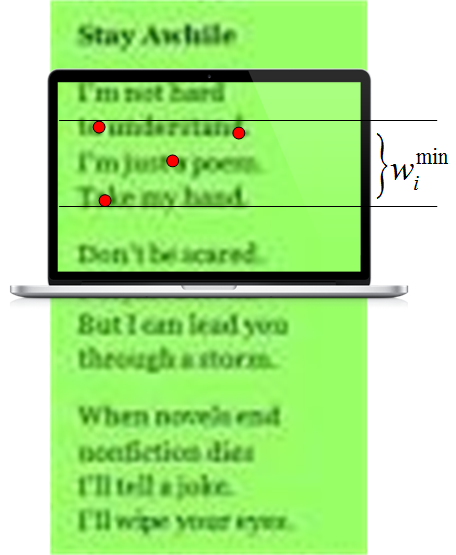
\includegraphics[width=0.7\columnwidth]{pictures/single_click}
\caption{Mouse click and reading region}
\label{fig:single_click}
\end{figure}


However, $w_i^{\min }$ is a minimum approximate of $w_i$, we can have a more accurate approximate if we take the neighboring 
scroll actions into consideration. In figure \ref{fig:neighbor_scroll}, we put the click data both before $i$th scroll(purple dots) and after $i+1$th(yellow dots).
We can see there is a gap between two neighbor minimum approximates($g1$ and $g2$ in figure\ref{fig:neighbor_scroll}). So we can have a moderate estimate of $w_i$:

\begin{equation} \label{eq:4}
{w_i} = w_i^{\min } + ({g_1} + {g_2})/2
\end{equation}

 
\begin{figure}[!h]
\centering
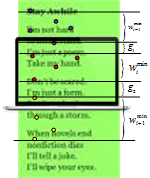
\includegraphics[width=0.9\columnwidth]{pictures/neighbor-scroll}
\caption{Mouse click and reading region}
\label{fig:neighbor_scroll}
\end{figure}


It should be noted that, ideally, $w_i^{\min } = {w_i} = {w_0}(1 \le i \le n)$ and 
$g_1=g_2=0$. But in fact, it is unlikely that a user starts reading and
finishes reading from the exact same locations, click data has to be considered
to compute RRR. If there is no click data available, we use BRR to replace RRR.

\section{ What and to what extent you have read}
Once we compute the BRR and RRR, we can answer our second research question: what and to what extents a user has read.
Here we want to answer this question in a finer granularity. We consider a whole article to be a bad granularity, instead, we 
answer this question to the granularity of paragraph.

 In order to formulate our solutions here, we introduce the following 
notations. Given two points $p_1(x_1,y_1)$ $p_2(x_2,y_2)$  on a screen at time instant $t$, the context identified by the two points can be 
notated as : $C(p_1,p_2)$, which is indicated as dark background texts in figure \ref{fig:context_points}. The corresponding time spent reading  
this context is $T(p_1,p_2)$.  

\begin{figure}[!h]
\centering
%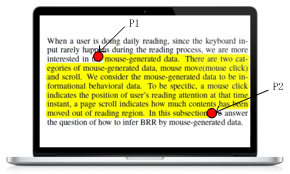
\includegraphics[width=0.9\columnwidth]{pictures/contexts-in-points}
\includegraphics[width=0.9\columnwidth]{pictures/scroll1}
\caption{Contexts between points}
\label{fig:context_points}
\end{figure}

For each scroll span $w_i$, $p_s$ is defined as the left top point of that screen area, $p_e$ is defined as the right bottom point of that screen area. Intuitively, 
we can have the reading time of  this screen $T(w_i)$ as follows:
\begin{equation} \label{eq:5}
T(w_i) = T(p_s,p_e)
\end{equation}

\begin{figure}[!h]
\centering
\includegraphics[width=0.9\columnwidth]{pictures/click-noise}
\caption{Mouse Click and Text Extraction}
\label{fig:click-noise}
\end{figure}

However, it is only a coarse-grid  estimation of the dwell time, because the context  $C(p_1,p_2)$ is relatively large. By taking the 
mouse click data into consideration, we can have a fine-grid estimation of dwell time. As we stated before, we consider mouse click 
as indication of real time user attention. However, there might be some "noise"  in mouse click data, which can not be considered as 
a clue of user reading. Figure \ref{fig:click-noise} illustrates a typical reading scenario where mouse click and mouse trajectory are 
displayed. Apparently, point/click $p_3$ is considered to be a "noise", since the position of $p_3$ does not indicate any text contents.
This might indicate a occasional subconscious click. Except $p_3$, all the  other six points locate in a certain text area. However, not all
of these six points can be used as reading attention indication.

 In real time, we note each click as  $k(t,x,y)$, where $t$ is timestamp, $x,y$ are the cooridnate of the point where click happened. 
The intentional click happens in a sequence of $k_1 k_2 k_3 ... k_n$. So, based on our assumption of line-by-line reading, we have the following equations 
hold, in equation \ref{eq:6}, $1 \le i < j < k \le n$.

\begin{equation} \label{eq:6}
\left\{ {\begin{array}{*{20}{c}}
{C({k_i},{k_j}) \cap C({k_l},{k_s}) = \emptyset }\\
{{t_i} < {t_j} \le{t_l} < {t_k}}
\end{array}} \right.
\end{equation}

According to equation \ref{eq:6} we can filter out $P_5$(in figure \ref{fig:context_points}) as noise since 
$C({k_1},{k_2}) \cap C({k_4},{k_5}) \ne \emptyset $. 

In practice, the information if a click is intentional or not is not given, so we developed algorithm \ref{algo:max}to find the maximal 
intentional click set(ICS) where equation \ref{eq:6} holds.

\begin{algorithm}
\DontPrintSemicolon % Some LaTeX compilers require you to use \dontprintsemicolon instead
\KwIn{The set of clicks $K=\{k_1, k_2, \ldots, k_n\}$}
\KwOut{The largest subset that fullfils equation \ref{eq:6} }


\For{$i \gets 1$ \textbf{to} $n$} {
    $S_i \gets  \{k_i\}   $\;
}

\For{$i \gets 1$ \textbf{to} $n$} {
	\If{ $S_i = \emptyset $  } {
		continue;
	}
	\For{$j \gets 1$ \textbf{to} $i-1$} {
    		\If{ ${S_j} \cup \{ {k_i}\}$ fulfills equation  \ref{eq:6} } {
			${S_j} \gets {S_j} \cup \{ {k_i}\} $
\\
			${S_i} \gets \emptyset$
		}
	}
}

$max \gets ||S_1||$\;

\For{$i \gets 1$ \textbf{to} $n$} {
	\If{ $||S_i|| > ||S_max||  $  }{
			$max \gets i$
	}
}

\Return{$S_{\max }$}\;
\caption{Find the maximal ICS(intentional click set)}
\label{algo:max}
\end{algorithm}



\section{Design and Implementation of UUAT}
To verify our ideas, we designed and implemented an Unobtrusive User Attention Tracking(UUAT) 
system, which can accomplish two tasks after collecting user behavioral data: 1.  Calculate the user reading region, 
BRR or RRR. 2. Infer what content(texts) and how long a user has read in an article. 
In this section we introduce our UUAT system and present our implementation details.

Since our goal is to analyze daily online reading, we prefer 
Browser-Client(BS) architecture to Client-Server(CS) architecture, for the reason that
BS architecture is more scalable and platform-independent. 
We choose browser plugin/extension as our implementation architecture, for the following considerations:
1. Compatability. The plugin technology has been supported by all the mainstream web browsers. 
2. Agility. The development cost and deployment cost of a plugin-based solution is very low. 
3. Privacy. All the collected data is under full control of a user himself. The user can keep all data at his own computer and analyze it locally, or he can choose a cloud service to analyze his data.


\begin{figure}[!h]
\centering
\includegraphics[width=0.9\columnwidth]{pictures/uuat_arch}
\caption{UUAT architecture}
\label{fig:uuat-arch}
\end{figure}

Figure \ref{fig:uuat-arch} illustrates the architecture of UUAT as a chrome plugin. Once user requested an article from a website, the
browser will first get the HTML contents for that article, then the html contents will be passed to UUAT and JavaScript code will be embedded into the original 
HTML page. When a user is reading this article, his behavioral data will be captured and saved at a local position. In real time, user behavior can be 
analyzed with the help of historical data(if there is historical data) and reading context data can be collected. 

UUAT collects three types of raw interaction data: MouseClick, Cursor and Scroll. The click and cursor are relatively easy to capture, by assigning handlers to $document.onclick$ and
$document.onmousemove$ event listeners, UUAT can easily log the position where the click happens and the cursor trajectory. The logging of user scroll is subtle. There are many 
cases (also in our collected data) a user scroll the screen more than one time in a very short time, during which no actual reading happened. 
Actually this happens very often when the user scrolls to a new position and aligns his reading region with the article contents before his scroll. 
To detect a real user scroll action, we adopted a look-backl strategy to rule out those "adjust-use" scrolls, which is shown in the following code piece.



\lstinputlisting{js_code.js}




\subsection{Behavioral Data Analysis} 
The goals of behavioral data analysis are twofold: 1. Combined with historical data, 
to calculate a preferred reading region so that  in the future when less behavioral data 
is provided, an estimation of user reading can still be calculated by historical reading 
model. 2. For this reading process, to calculate what a user have read and to what extent he has read. 


\section{Experiment and Verification}




\subsection{Experimental Design and Procedure}




 




\bibliographystyle{acm-sigchi}
\bibliography{sample}
\end{document}
